\newpage

\section{Network Topology and Architecture}

This section presents the network topology designed for the SoftEther VPN laboratory activity. The implementation simulates a realistic scenario where two geographically separated private networks communicate securely across the Internet through VPN tunnels. 

\subsection{Topology Overview}

The laboratory network topology consists of five main components that work together to create a realistic Internet-based VPN scenario:

\begin{figure}[H]
\centering
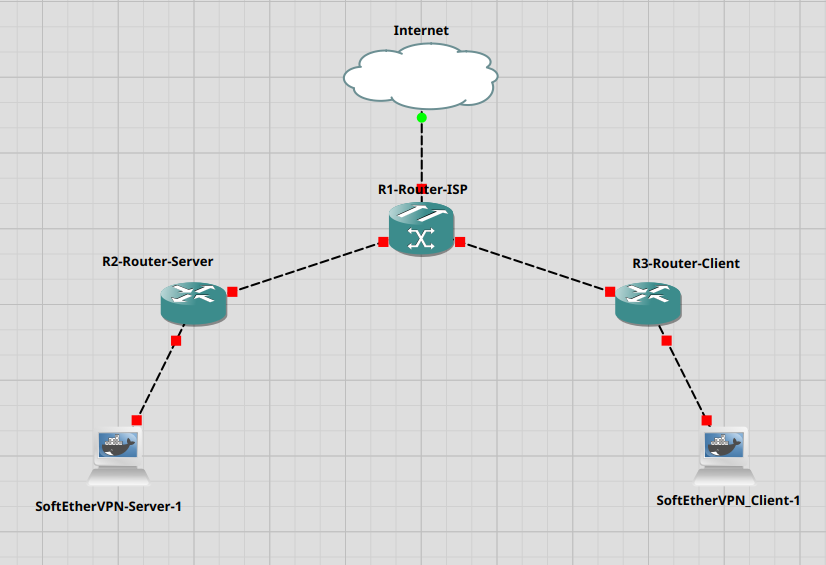
\includegraphics[width=0.9\textwidth]{../resources/Images/GNS3_Structure.png}
\caption{GNS3 Network Topology - VPN Across the Internet}
\label{fig:gns3_topology}
\end{figure}

The network architecture follows an end-to-end VPN design where:

\begin{itemize}
    \item \textbf{Server Site:} Contains the SoftEther VPN server hosted within a private network
    \item \textbf{Client Site:} Represents a remote branch office requiring VPN connectivity
    \item \textbf{Internet Infrastructure:} Simulated ISP network providing public connectivity
    \item \textbf{Edge Routers:} Perform NAT and routing functions, providing Internet connectivity for the private networks
    \item \textbf{VPN Endpoints:} Docker containers hosting the actual VPN software 
\end{itemize}

This topology effectively demonstrates how end-to-end VPN technology enables secure communication between hosts in different private networks across untrusted public infrastructure, representing common real-world deployment scenarios where VPN software runs directly on the endpoints rather than on gateway devices.

\subsection{IP Addressing Scheme}

The network addressing scheme uses a combination of private and public IP addresses to simulate realistic Internet connectivity. The addressing follows RFC standards for private addressing (RFC 1918) and uses documentation addresses (RFC 5737) for public IP simulation.

\begin{table}[H]
\centering
\caption{Network Interface Configuration}
\label{tab:ip_addressing}
\begin{tabular}{|l|l|l|l|}
\hline
\textbf{Device} & \textbf{Interface} & \textbf{IP Address} & \textbf{Description} \\
\hline
\multirow{2}{*}{Router 2 (Server-side)} & LAN (Fa0/0) & 10.0.1.1/24 & Private Network 1 \\
 & WAN (Fa0/1) & 203.0.113.1/24 & Public IP (RFC 5737) \\
\hline
\multirow{3}{*}{ISP Router} & Interface Fa0/0 & 203.0.113.254/24 & Connected to Router 2 \\
 & Interface Fa0/1 & 198.51.100.254/24 & Connected to Router 3 \\
 & Interface Fa1/0 & DHCP Assigned & Internet Cloud \\
\hline
\multirow{2}{*}{Router 3 (Client-side)} & WAN (Fa0/1) & 198.51.100.1/24 & Public IP (RFC 5737) \\
 & LAN (Fa0/0) & 10.0.2.1/24 & Private Network 2 \\
\hline
SoftEther Server & eth0 & 10.0.1.2/24 & VPN Server Host \\
\hline
VPN Client & eth0 & 10.0.2.2/24 & VPN Client Host \\
\hline
\end{tabular}
\end{table}

\textbf{Network Segments:}

\begin{itemize}
    \item \textbf{Server Network (10.0.1.0/24):} Private subnet hosting the SoftEther VPN server
    \item \textbf{Client Network (10.0.2.0/24):} Remote private subnet with VPN client
    \item \textbf{ISP Segment 1 (203.0.113.0/24):} Public network between ISP and server-side 
    \item \textbf{ISP Segment 2 (198.51.100.0/24):} Public network between ISP and client-side 
    \item \textbf{VPN Tunnel Networks:} Virtual addressing for VPN connectivity (assigned dynamically)
\end{itemize}

\subsection{Device Roles and Functions}

Each component in the network topology serves a specific purpose in demonstrating VPN functionality:

\subsubsection{ISP Router (R1-Router-ISP)}

The ISP router simulates Internet Service Provider infrastructure and provides:

\begin{itemize}
    \item \textbf{Internet Connectivity:} DHCP-assigned public IP address with MAC address spoofing for network access (Explained later).
    \item \textbf{Inter-Site Routing:} Routes traffic between the two remote sites through simulated Internet infrastructure
    \item \textbf{NAT Traversal Support:} Enables VPN protocols to function through Network Address Translation
    \item \textbf{Public IP Assignment:} Provides public addressing for both edge routers
\end{itemize}

The ISP router configuration includes static routes for both private networks and implements a default route to the Internet cloud.

\subsubsection{Server-Side Router (R2-Router-Server)}

This edge router connects the server's private network to the Internet and implements:

\begin{itemize}
    \item \textbf{Network Address Translation:} Port Address Translation management
    \item \textbf{VPN Port Forwarding:} Static NAT rules to forward VPN traffic to the server:
    \begin{itemize}
        \item Port 500/UDP: ISAKMP forwarded to SoftEther server
        \item Port 4500/UDP: NAT-T forwarded to SoftEther server
        \item Port 443/TCP: HTTPS/TLS forwarded to SoftEther server
    \end{itemize}
    \item \textbf{Default Gateway:} Routing for the server's private network
    \item \textbf{Transparent Routing:} Routes VPN traffic between Internet and private network without VPN processing
\end{itemize}

\subsubsection{Client-Side Router (R3-Router-Client)}

The client-side edge router provides similar functionality for the remote site:

\begin{itemize}
    \item \textbf{PAT Configuration:} Network address translation for client network connectivity
    \item \textbf{Default Routing:} Internet access for the client private network
    \item \textbf{Transparent VPN Support:} Allows VPN client software to establish connections through NAT without router-based VPN processing
\end{itemize}

\subsubsection{SoftEther VPN Server Container}

The server container runs the SoftEther VPN software with the following configuration:

\begin{itemize}
    \item \textbf{Container Image:} \texttt{siomiz/softethervpn:latest}
    \item \textbf{Multi-Protocol Support:} Simultaneous IPSec and TLS/SSL VPN services
    \item \textbf{Virtual Hub:} DEFAULT hub for client connections
    \item \textbf{User Management:} Configured with test user accounts for VPN authentication
    \item \textbf{Certificate Management:} Self-signed certificates for TLS-based connections
\end{itemize}

\subsubsection{VPN Client Container}

The client container simulates a remote user or branch office with:

\begin{itemize}
    \item \textbf{Container Image:} \texttt{ubuntu:latest}
    \item \textbf{IPSec Client:} StrongSwan software for IPSec connectivity
    \item \textbf{TLS Client:} OpenVPN client for SSL/TLS VPN connections
\end{itemize}

\subsection{Network Communication Flow}

The network design enables several communication scenarios:

\begin{enumerate}
    \item \textbf{Direct Internet Communication:} Both sites can access Internet resources through their respective ISP connections
    
    \item \textbf{End-to-End VPN Tunnel Establishment:} The VPN client container initiates direct VPN connections to the SoftEther server container using either:
    \begin{itemize}
        \item IPSec protocol (strongSwan client to SoftEther server)
        \item TLS/SSL protocol (OpenVPN client to SoftEther server)
    \end{itemize}
    
    \item \textbf{Encrypted Inter-Site Communication:} Once VPN tunnels are established, the client can communicate securely with resources in the server's network
    
    \item \textbf{NAT Traversal:} VPN protocols handle NAT traversal automatically, allowing encrypted tunnels to pass through the edge routers
\end{enumerate}

\subsection{Security Considerations}

The network topology incorporates several security features:

\begin{itemize}
    \item \textbf{Private Addressing:} Internal networks use RFC 1918 private addresses, preventing direct Internet access
    \item \textbf{NAT Protection:} Edge routers provide implicit firewall protection through NAT
    \item \textbf{VPN Encryption:} All inter-site communication is protected by VPN encryption
    \item \textbf{Authentication:} VPN connections require user credentials and/or certificates
    \item \textbf{Protocol Separation:} Different VPN protocols operate on distinct ports for protocol isolation
\end{itemize}

This topology provides a foundation for comparing different VPN implementations while maintaining realistic network security practices and demonstrating practical deployment scenarios.
